\section*{Introduction}

% the separation of sections here is artificial, the body does not have an intro, results nor outro

The $\Lambda$CDM cosmological model has proven extremely effective in
predicting the evolution of our Universe, relying on only six parameters
\cite{Planck2020a}.
In particular, it explains the transition from a predominantly neutral
state in the early stages to the familiar ionized intergalactic medium
(IGM) observed in our relatively nearby surroundings.
This transition is known as cosmic reionization.
Despite a comprehensive understanding of the astrophysical principles
governing this transition, uncertainties persist regarding its precise
timeline \cite{Jin2023}.
The advent of the James Webb Space Telescope (JWST) \cite{Gardner2006}
represents a pivotal moment, substantially bolstering our ability to
directly constrain the evolution of the neutral hydrogen fraction
$x_\HI$.
This progress is being driven by the JWST's enhanced detection
capabilities, enabling the observation of high-redshift quasars
\cite{Eilers2023} and high-redshift galaxies
\cite{Adams2023, Bradley2023, Donnan2023}.

Reionization leads to scattering of Cosmic Microwave Background (CMB)
photons by free electrons, disrupting the CMB angular power spectra
($C_\ell$).
This scattering suppresses the signal at scales smaller than the Hubble
scale at reionization (approximately $\ell>10$) \cite{Planck2020b} due
to the increased\YLtodo{nonzero?} optical depth $\tau_\reio$.
Additionally, it introduces a new signal in the polarization of CMB
photons at large angular scales \cite{Planck2020a}, that is $\propto
\tau_\reio$ in $C^{TE}_\ell$, the cross-correlation of the $E$-mode
polarization with the temperature (intensity), and is $\propto
\tau_\reio^2$ in $C^{EE}_\ell$, the $E$-mode polarization angular auto
power spectrum.
Consequently, heightened sensitivity to CMB polarization becomes crucial
for mitigating the degeneracy between $\tau_\reio$ and other
cosmological parameters, particularly $\As$, the amplitude of the
primordial scalar power spectrum, and $r$, the ratio of tensor-to-scalar
modes \cite{Natale2020}.

While the high-$\ell$ signal holds most of the constraining power for
cosmological parameters, the low-$\ell$ polarization is crucial for
accurately determining $\tau_\reio$.
Hence\YLtodo{connection not obvious to me}, breaking the degeneracy with $\As$ and diminishing\YLtodo{can diminish?} the influence
of $\tau_\reio$ on other anomalous parameters like $A_\mathrm{lens}$
\cite{Giare2023}.
$A_\mathrm{lens}$ contains information about the expected deflection of
CMB photons due to the underlying matter distribution.
However, interpreting signals at large angular scales (low $\ell$)
without affecting high-$\ell$ measurements has proven challenging.
\YLtodo[inline]{need to ask Paulo more about these 2 sentences}
This challenge may ultimately require adopting a comprehensive Bayesian
framework to jointly consider cosmology, astrophysics, and instrument
systematics \cite{Paradiso2023}.
\autoref{fig:tau} illustrates current representative constraints on
$\tau_\reio$.\YLtodo{feels a bit out of place here}

\begin{figure}
\centering
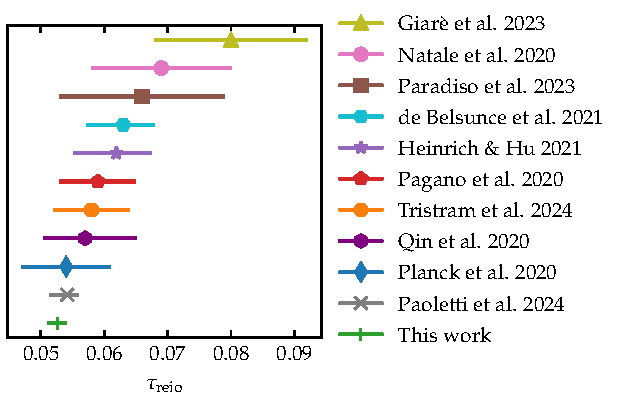
\includegraphics{figs/tau_fig.pdf}
\caption{\textbf{Current constraints on the optical depth to
reionization ($\tau_\reio$) from Cosmic Microwave Background (CMB)
data.}
The error bars indicate the 1$\sigma$ uncertainties.
Various analyses may employ distinct data sets or vary in the parameters
considered.
For instance, the inclusion of WMAP data in Refs.
\cite{Natale2020, Paradiso2023} (circle and square) or ACT in
combination with other external data sets \cite{Giare2023} (triangle),
expanded sky coverage \cite{Paradiso2023} (square), incorporation of
high-$\ell$ data \cite{Pagano2020, Planck2020a, Giare2023} (pentagon,
star, and triangle),
marginalization over small set of strongly correlated parameters
\cite{Natale2020} (circle), and the implementation of an end-to-end
Bayesian framework that marginalizes over astrophysics and instrumental
systematics \cite{Paradiso2023} (square).}
\label{fig:tau}
\end{figure}

Given the challenges posed by $\tau_\reio$ in CMB analyses and the
anticipated advancements in constraining the reionization timeline
\cite{Montero2021, Hera2022}, now is an opportune moment to reassess its
role.
Cosmic reionization should be uniquely determined given a specific
cosmology, i.e.\ by the other five cosmological parameters.
Specifically, the evolution of the global fraction of neutral hydrogen
can be written as
%
\begin{equation}
\label{eq:premise}
x_\HI = f(\sigma_8, \ns, h, \Omegab, \Omegam) \quad \Rightarrow \quad
\tau_\reio = g(\sigma_8, \ns, h, \Omegab, \Omegam),
\end{equation}
%
where $\ns$, $h$, $\Omegab$, and $\Omegam$ are the tilt of the
primordial power spectrum, dimensionless Hubble constant, and present
baryon and matter densities, respectively.
$\sigma_8$ is the present linear rms relative density fluctuation in a
sphere of radius $8 h^{-1}$ Mpc.
In principle, This parametrization chosen for convenience fully
determines $x_\HI$, but the incomplete understanding of cosmic
reionization complicates this mapping, necessitating the introduction of
$\tau_\reio$ in CMB analyses.
However, our understanding of the astrophysical processes governing
reionization has significantly improved
\cite{Gnedin2022, Kannan2022, Murray2020, Fan2023} since the inclusion
of $\tau_\reio$ became a standard practice.
Ongoing and forthcoming observations promise to further refine our
understanding and reduce inherent modeling uncertainties.
Motivated by these developments, we use symbolic regression (SR)
\cite{Cranmer2023} to construct a mapping between cosmology and
reionization timeline, aiming to demote $\tau_\reio$ from an independent
to a derived cosmological parameter.

Accurately measuring the optical depth to reionization could
significantly enhance tighten CMB parameter constraints, especially as
$\tau_\reio$ remains the only independent cosmological parameter not
constrained to sub-percent precision \cite{Planck2020b}.
To achieve this precision, sensitivity to E-mode polarization at levels
of $\lesssim 10^{-2} \ \mu$K$^2$ and meticulous control of systematic
effects and foregrounds residuals are essential.

Eq.~(\ref{eq:premise}) introduces a novel avenue to constrain cosmology
by examining the dependence of $x_\HI(z)$ on cosmological parameters.
This mapping can enhance parameter constraints and shed light on
reionization astrophysics.
It also aids ongoing efforts in parametrizing cosmic reionization models
\cite{Trac2018, Trac2022} by including the cosmological dependence of
$x_\HI$.


\section*{Results}

Here, we present a universal shape for the evolution of the neutral
hydrogen as a function of cosmology, derived through SR on simulated
reionization histories from 21cmFAST \cite{Murray2020}.
We integrate this shape into CLASS \cite{Blas2011}, a popular Boltzmann
solver for CMB analyses.
We then evaluate the modified CLASS alongside cobaya \cite{Torrado2020},
a speed-aware sampler\footnote{With fast-dragging as in
\cite{Neal2005}.} \cite{Lewis2002, Lewis2013}, showcasing its ability to
recover parameter constraints from CMB data, including `TTTEEE' +
lensing likelihoods \cite{Planck2020c, Planck2020d} (see
\autoref{fig:tg}).
Finally, we demonstrate cosmological gains by computing $\tau_\reio$ as
a derived parameter using our approach -- Eq.~(\ref{eq:premise}) --
compared to sampling over $\tau_\reio$ using the conventional $\tanh$
model \cite{Lewis2008}.
We summarize our strategy in \autoref{fig:big}.

\begin{figure}
\centering
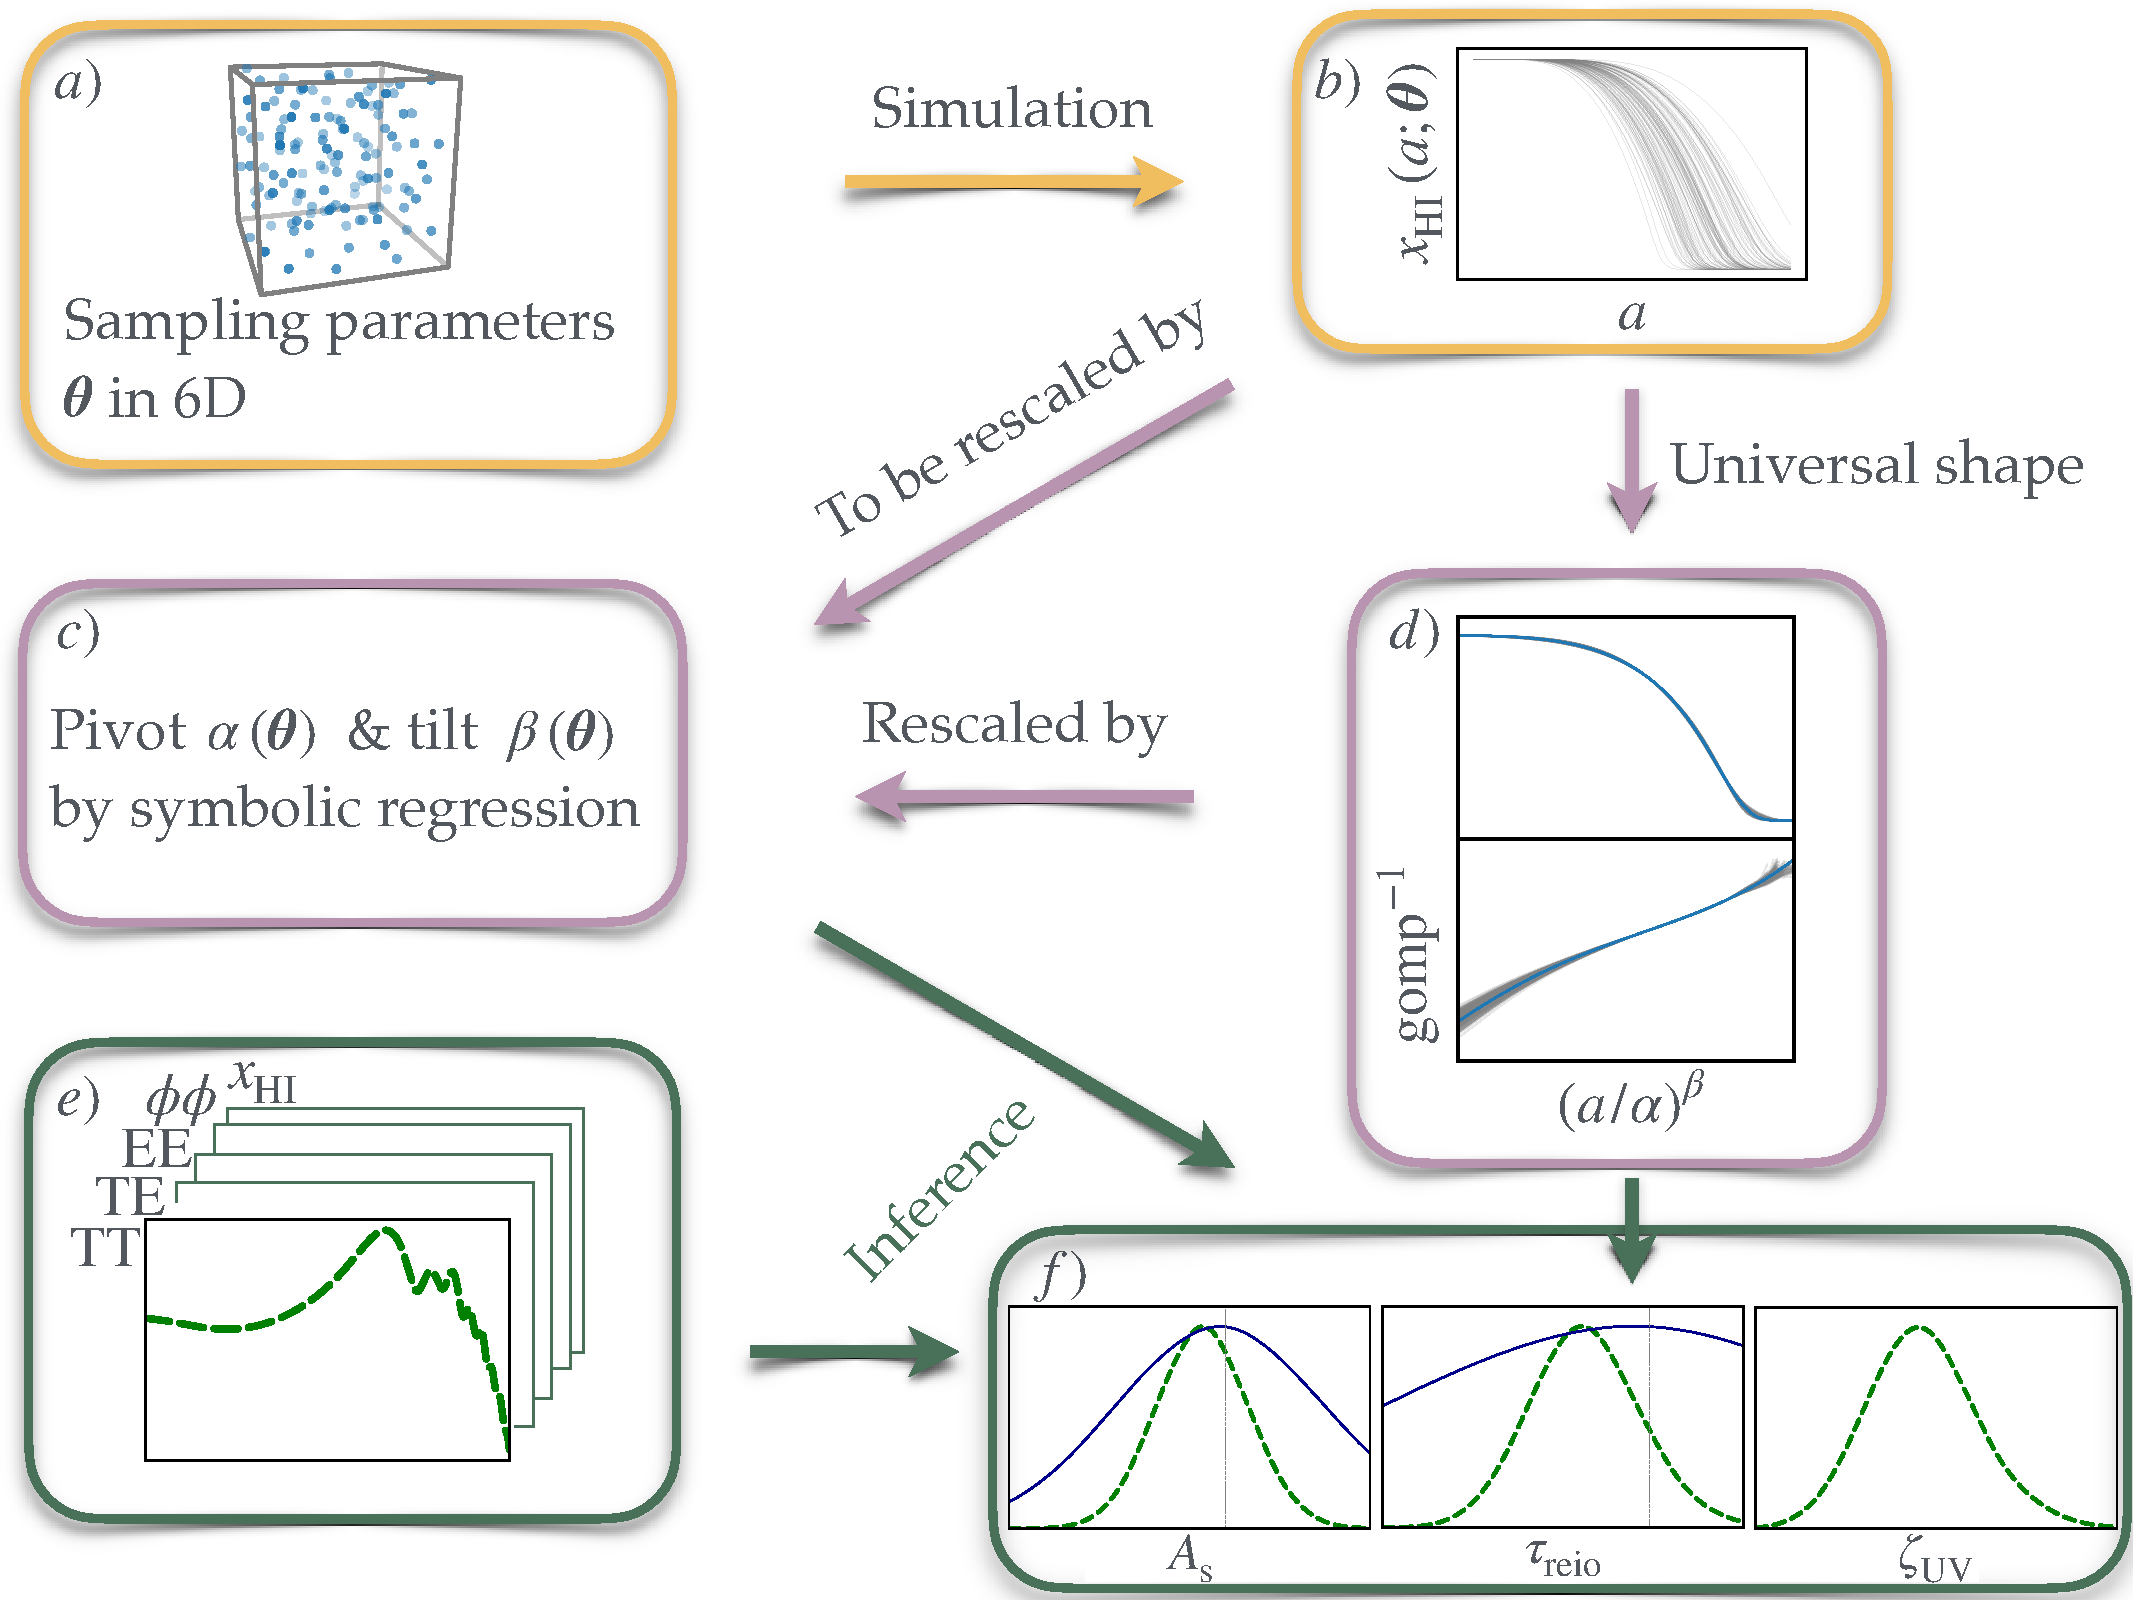
\includegraphics[width=\linewidth]{figs/big_fig.pdf}
\caption{\textbf{Strategy to demote $\tau_\reio$ to derived parameter.}
\emph{a)} Sobol sampling of 5 cosmological parameter and 1 astrophysical
one (see \autoref{fig:sobol} in extended data).
\emph{b)} Generated $x_\HI$ profiles as a function of scale factor and
sampled parameters.
\emph{c)} We determine the mapping, i.e.\ the rescale, between
parameters and $x_\HI$ profiles using symbolic regression.
\emph{d)} A universal shape is computed using the rescale and the
Gompertz curve.
The lower panel showcases the distribution of the residuals, we fit the
residuals with a six-degree polynomial.
\emph{e)}  CMB angular power spectra.
The model prediction is obtained using classy while the observational
data comes from the Planck likelihoods.
\emph{f)} We use cobaya to make the inference using Monte Carlo Markov
Chain sampler.}
\label{fig:big}
\end{figure}

To achieve our goal outlined in Eq.~(\ref{eq:premise}), we construct a
universal shape for $x_\HI$.
All $x_\HI(z)$ profiles share this shape, with differences between
scenarios being mere rescalings or translations.
Reionization causes $x_\HI$ to transition from near 1 to effectively 0,
making a sigmoid function suitable.
The asymmetric nature of reionization history
\cite{Trac2018, Doussot2019} suggests a Gompertz curve might be better
suited than a symmetric $\tanh$ transition, providing an early start and
rapid completion.
The Gompertz curve, often used to model age-dependent human mortality
\cite{Gompertz1825}, fulfills the requirements as a sigmoid function
with the desired asymmetry.

The foundational principle behind the universal shape for $x_\HI$ is
treating it as a cumulative probability distribution.
This insight allows us to handle its derivative with respect to $y$ as a
probability density function (PDF), where $y = \ln\ar$ represents both
time evolution and peak location.
This PDF should apply to different reionization scenarios, although its
pivot and tilt may depend on cosmology.
Therefore, $\ar$ acts as a rescaled scale factor mapping cosmological
parameters to reionization history.
We demonstrate this rescale in \autoref{fig:shape} in the extended data.
Essentially, cosmology impacts the \emph{mean} of the distribution, not
its shape.

To enhance the flexibility of our Gompertz curve, we introduce a
six-degree polynomial in $\ln\ar$ to reduce residuals and improve the
separation of time evolution from cosmological dependence.
This combined approach, using Gompertz and the PDF perspective,
parametrizes the evolution of HI as follows
%
\begin{align}
\label{eq:uni}
x_\HI(\ar) &= \Gomp\bigl( P_5(\ar) \bigr)
  \equiv \exp\bigl[ - \exp\bigl( P_5(\ar) \bigr) \bigr], \\
%
\label{eq:map}
\ar(a; \vtheta) &= \Bigl[ \frac{a}{\ap(\vtheta)} \Bigr]^\tilt ,\\
%
\label{eq:poly}
P_5(\ar) &= {\textstyle\sum}_{m=0}^5 \, c_m \ln^m\!\ar, \\
%
\nonumber
\bm{c} &= \{0, 1, 0.1503, 0.04850, 0.005261, 0.0002182\},
\end{align}
%
\YLtodo{number of sig figs}
where $\vtheta$ corresponds to cosmological parameters, $\ap(\vtheta)$
represents the pivot of the rescaling, and $\tilt = 8.290$ is the
rescaling tilt, which, according to our 21cmFAST simulations, appears
constant.
This lack of cosmological dependence may stem from 21cmFAST's treatment
of reionization astrophysics.
See \ref{ssec:helium} for specifics on implementing HeI and HeII
reionization.\PMCtodo{What do you mean by sig here?}

Before fully leveraging our formalism to extract the cosmological
dependence in the rescale of Eq.~(\ref{eq:uni}) and potentially
eliminating the need for $\tau_\reio$ in CMB analyses, we first
implement the Gompertz shape in CLASS and confirm its agreement with the
conventional $\tanh$ model.
Using Planck 2018 likelihoods `TTTEEE' \cite{Planck2020c} and CMB
lensing \cite{Planck2020d}, we sample typical cosmological parameters
with cobaya \cite{Torrado2020}, including $\tau_\reio$.
The sampler runs until the Gelman-Rubin statistic \cite{Lewis2013}
satisfies $R - 1 < 0.2$ for the between-chain variance of the confidence
intervals.
We repeat this for $\tanh$ reionization.
Sampling over $\tau_\reio$ implies that CLASS finds the reionization
history producing the desired optical depth using bisection.
For $\tanh$ reionization, this varies the midpoint, while for Gompertz,
it varies the pivot in the rescale, $\ln\ap$, to match the input
$\tau_\reio$.

\autoref{fig:tg} and Table \ref{tab:tau_comp} in the extended data
summarize the recovery experiment.
The only notable differences in inferred parameters are in the midpoint
of reionization $z_\re$.
The Gompertz scenario suggests a more delayed reionization by over
$1\sigma$, with $z_\re = 6.81 \pm 0.68$ compared to $7.67 \pm 0.75$ for
the $\tanh$ model.
Our results align with recent high-$z$ quasar observations
\cite{Keating2020}.
All other cosmological parameters are in good agreement with Planck's
results \cite{Planck2020a}, with errors of $\lessapprox 0.4 \%$.

Having confirmed that the mortality-based reionization can reproduce
standard CMB analyses, we aim to establish the connection between the
universal shape for $x_\HI$ and the rescaling of  a given reionization
scenario.
This rescaling is naturally a function of cosmology.
For example, a larger density of matter $\Omegam$ results in deeper
potential wells, accelerating structure formation and increasing the
number of ultraviolet photons driving the reionization process.
To confirm the universality of our Gompertz reionization and its
cosmology dependence, we use 126 Sobol samples of 21cmFAST simulations
(see \ref{ssec:sims} and \autoref{fig:sobol} in the extended data)
and employ PySR, a SR package, to extract the cosmological dependence of
the rescaling in Eq.~(\ref{eq:map}).

While PySR initially guided us towards the Gompertz mortality law, the
final analysis only uses it to regress the pivot of the rescaling.
We input Eq.~(\ref{eq:uni}) to the genetic algorithm and find the pivot
that best (see \ref{ssec:pysr} in extended data for our definition of
\emph{best}) matches the reionization histories in our 128 21cmFAST
simulations to the Gompertz curve.
Using PySR we derived the following rescaling as a function of cosmology
%
\begin{equation}
\label{eq:SR}
\ln\ap(\vtheta) = (h^{\Omegam} + \sigma_8) (\Omegab - \ns - \Omegam).
\end{equation}

Eqs.~(\ref{eq:map},\ref{eq:SR}) imply that higher values of $\ns$ hasten
reionization by boosting power on small scales, fostering a greater
abundance of ionizing sources and earlier completion \cite{Montero2021}.
Note that our 21cmFAST simulations assume that faint galaxies are the
primary drivers of reionization.
Similarly, larger $\Omegam$ and $\sigma_8$ primarily expedite
reionization by enhancing structure formation.
Surprisingly, Eq.~(\ref{eq:SR}) suggests that higher $\Omegab$ delays
reionization, likely due to the increased abundance of HI in the
intergalactic medium requiring more ionizing photons.

We note that within the prior range of our 21cmFAST simulations (see
\ref{ssec:sims}) and their corresponding astrophysics of reionization,
the mapping derived from SR is not unique.
Additional details and results using an alternative mapping are
presented in \ref{ssec:0226} of the extended data.

We implement Eq.~(\ref{eq:SR}) in our Gompertz CLASS.
If the input excludes $\tau_\reio$, the algorithm determines the rescale
and consequently the reionization history, $\tau_\reio$, and
corresponding CMB angular power spectra using the cosmological
parameter.
This eliminates the need to sample over $\tau_\reio$ (or $z_\re$),
requiring only five cosmological parameters.
We use cobaya to re-analyze the same Planck likelihoods, showcasing the
full strength of our approach.

\begin{figure}
\centering
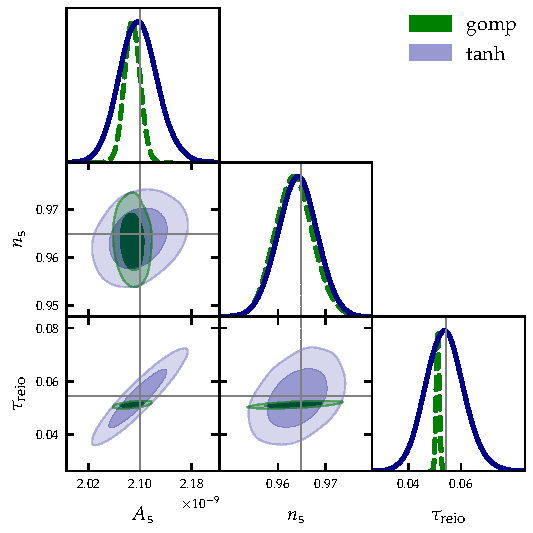
\includegraphics[width=\linewidth]{figs/gomp_tanh_triangle_kill.pdf}
\caption{\textbf{Analysis of CMB data with reionization as a function of
cosmology.}
\YLtodo[inline]{contour and PDFs look quite big}
The green contours represent our results using the Gompertz reionization
scenario with Eq.~(\ref{eq:SR}), eliminating the need to sample over any
reionization parameter.
The blue contours correspond to the results obtained using the
conventional $\tanh$ model, while the relevant Planck constraints
\cite{Planck2020a} are depicted with gray lines for reference.}
\label{fig:kill}
\end{figure}

\autoref{fig:kill} underscores the impact of our mortality-based
reionization scenario.
The Gompertz scenario does not sample over reionization parameters but
maps cosmology parameters to $x_\HI$ profiles.
This approach improves the constraint on the optical depth to $\approx
1\%$, a remarkable improvement compared to $> 10\%$ with the $\tanh$
prescription.
Furthermore, the constraint on $\As$ improves drastically since the TT
data is no longer significantly hampered by the degeneracy between $\As$
and $\tau_\reio$.
The error on $\As$ decreases by an impressive 2.5 compared to Planck's
results\cite{Planck2020a}.
Overall, we recover tighter constraints across the board compared to
Planck.
See Table \ref{tab:para} in the extended data for details.


\section*{Outro}

\begin{figure}
\centering
\includegraphics[width=\linewidth]{figs/history.pdf}
\caption{\textbf{Reionization history.}
The $x_\HI$ profile based on the best-fit values from our Gompertz
reionization scenario applied to Planck data (green dashed line).
We also include an alternative mapping from cosmology to reionization
timeline in the pink dashed line (see \ref{ssec:0226}).
The $\tanh$-based Planck constraint is also shown (blue line).
Additionally, we include observational constraints from high-redshift
quasars \cite{Greig2017, Banados2018, Davies2018, Greig2019, Wang2020,
Yang2020, Greig2022, Jin2023} and galaxies \cite{Ouchi2010,
Sobacchi2015, Mason2018, Mason2019, Hoag2019, Mesinger2015}.}
\label{fig:history}
\end{figure}

Our results suggest that Planck data favors a delayed reionization
compared to other CMB-based constraints.
Our best-fit cosmological parameters indicate a midpoint of $z_\re =
7.40$ and a duration of $\Delta z \equiv z(x_\HI = 0.05) - z(x_\HI =
0.95) \sim 500 $ Myr.
While our results align with late reionization observations, the
difference with the $\tanh$ model is within 1$\sigma$.
The duration of reionization, though better suited to observational
constraints compared to the $\tanh$ model, might still be considered
somewhat rapid in the context of late reionization scenarios (see
\cite{Cain2021}).
\autoref{fig:history} illustrates the reionization timeline derived
from our best-fit values.

Our findings for the timeline of reionization align with late
reionization scenarios, which are supported by high-$z$ Lyman-$\alpha$
observations \cite{Keating2020, Cain2021}.
However, recent discoveries by JWST indicate the presence of massive,
bright galaxies at early redshifts $z \sim 10$
\cite{Adams2023, Bradley2023, Donnan2023}.
The presence of these early galaxies suggests a potential preference for
brighter galaxies to drive reionization, a role that in our 21cmFAST
simulations was attributed to a population of faint galaxies.

Furthermore, our results are influenced by the semi-numerical
prescription employed by 21cmFAST to ionize the IGM, which, while
efficient and swift, could bias our findings.
Moreover, our exploration within the astrophysical framework of 21cmFAST
has been limited to varying the ionization efficiency (see
\ref{ssec:sims} in the extended data).
Therefore, a more comprehensive exploration is warranted to ensure, for
instance, that the tilt of the rescale remains a constant.
Additionally, a valuable exercise to refine the inherent relationship
between cosmological parameters and reionization history would involve
using more realistic, albeit slower, reionization models.
One such option is to use the THESAN simulations \cite{Kannan2022},
which are hydrodynamical simulations incorporating radiation transfer.


\paulo{Around 2000 words.}

\paulo{Body can only have 50 citations.}
